%% ===========================================================
%%  Beamer Presentation — Introduction to Neural Networks
%%  AIMS Rwanda, Kigali  |  March 2026
%%  Group 3: Object Detection with YOLOv5 on Pascal VOC 2012
%% ===========================================================
\documentclass[aspectratio=169, 10pt]{beamer}

%% ---------- packages ----------
\usepackage[T1]{fontenc}
\usepackage[utf8]{inputenc}
\usepackage{lmodern}
\usepackage{xcolor}
\usepackage{graphicx}
\usepackage{booktabs}
\usepackage{array}
\usepackage{tabularx}
\usepackage{amsmath, amssymb}
\usepackage{tikz}
\usepackage{microtype}

\usepackage{listings}
\usepackage{pgfplots}
\pgfplotsset{compat=1.18}

%% ---------- colours ----------
\definecolor{aimsblue}{RGB}{0, 70, 127}
\definecolor{aimsgold}{RGB}{204, 153, 0}
\definecolor{lightgray}{RGB}{245, 245, 245}
\definecolor{midgray}{RGB}{100, 100, 100}
\definecolor{darkbg}{RGB}{20, 30, 48}
\definecolor{codebg}{RGB}{230, 235, 245}

%% ---------- Beamer theme ----------
\usetheme{Madrid}
\usecolortheme[named=aimsblue]{structure}

\setbeamercolor{title}{bg=aimsblue, fg=white}
\setbeamercolor{frametitle}{bg=aimsblue, fg=white}
\setbeamercolor{block title}{bg=aimsblue, fg=white}
\setbeamercolor{block body}{bg=lightgray, fg=black}
\setbeamercolor{block title alerted}{bg=aimsgold, fg=white}
\setbeamercolor{block body alerted}{bg=lightgray, fg=black}
\setbeamercolor{itemize item}{fg=aimsblue}
\setbeamercolor{itemize subitem}{fg=aimsgold}
\setbeamercolor{enumerate item}{fg=aimsblue}
\setbeamercolor{footline}{bg=aimsblue, fg=white}
\setbeamercolor{headline}{bg=aimsgold}
\setbeamercolor{section in head/foot}{bg=aimsblue, fg=white}
\setbeamercolor{subsection in head/foot}{bg=aimsgold, fg=white}
\setbeamercolor{author in head/foot}{bg=aimsblue, fg=white}
\setbeamercolor{title in head/foot}{bg=aimsgold, fg=white}
\setbeamercolor{date in head/foot}{bg=aimsblue, fg=white}

\setbeamertemplate{navigation symbols}{}
\setbeamerfont{frametitle}{series=\bfseries}
\setbeamerfont{block title}{series=\bfseries}

%% ---------- gold rule under frametitle ----------
\addtobeamertemplate{frametitle}{}{%
  \vspace{-4pt}%
  {\color{aimsgold}\hrule height 1.5pt}%
  \vspace{2pt}%
}

%% ---------- listings setup ----------
\lstset{
  backgroundcolor=\color{codebg},
  basicstyle=\ttfamily\scriptsize,
  keywordstyle=\color{aimsblue}\bfseries,
  commentstyle=\color{midgray}\itshape,
  stringstyle=\color{aimsgold},
  breaklines=true,
  frame=single,
  rulecolor=\color{aimsblue},
  framesep=4pt,
  xleftmargin=5pt,
  xrightmargin=5pt,
}

%% ---------- metadata ----------
\title[Object Detection: Group 3]{%
  \textbf{Object Detection with YOLOv5}\\
  \large on the Pascal VOC 2012 Dataset}
\subtitle{Introduction to Neural Networks, Assignment II}
\author[Group 3]{%
  \textbf{Group 3}\\[2pt]
  \small Olusola Timothy Ogundepo \quad Lillian Mutesi\\
  \small Lucas Mirija Razafimanantsoa \quad Alliance Irigenera}
\institute[AIMS Rwanda]{%
  African Institute for Mathematical Sciences\\
  AIMS Rwanda, Kigali}
\date{March 2026}

%% ===========================================================
\begin{document}

%% -------- Title frame ----------------------------------------
\makeatletter
\begin{frame}[plain, t]
  \vspace*{-0.4cm}%
  \noindent\hspace*{-\beamer@leftmargin}%
  \begin{beamercolorbox}[wd=\paperwidth, ht=2.2cm, dp=0pt, center, sep=0.65cm]{section in head/foot}
    {\bfseries\normalsize African Institute for Mathematical Sciences \textbar\ AIMS Rwanda}
  \end{beamercolorbox}%
  \par\nointerlineskip
  \noindent\hspace*{-\beamer@leftmargin}%
  \begin{beamercolorbox}[wd=\paperwidth, ht=0.28cm, dp=0pt]{title in head/foot}
  \end{beamercolorbox}%
  \vspace{0.7cm}
  \begin{center}
    {\color{aimsblue}\LARGE\bfseries Object Detection with YOLOv5}\\[5pt]
    {\large\color{midgray} on the Pascal VOC 2012 Dataset}\\[10pt]
    {\color{aimsgold}\normalsize\itshape Introduction to Neural Networks --- Assignment II}\\[16pt]
    {\small\bfseries Group 3}\\[4pt]
    {\small Olusola Timothy Ogundepo \quad Lillian Mutesi}\\[2pt]
    {\small Lucas Mirija Razafimanantsoa \quad Alliance Irigenera}
  \end{center}
  \vfill
  \noindent\hspace*{-\beamer@leftmargin}%
  \begin{beamercolorbox}[wd=\paperwidth, ht=0.28cm, dp=0pt]{title in head/foot}
  \end{beamercolorbox}%
  \par\nointerlineskip
  \noindent\hspace*{-\beamer@leftmargin}%
  \begin{beamercolorbox}[wd=\paperwidth, ht=0.9cm, dp=0pt, center, sep=0.2cm]{section in head/foot}
    {\small\bfseries March 2026}
  \end{beamercolorbox}%
\end{frame}
\makeatother

%% -------- Outline -------------------------------------------
\begin{frame}{Outline}
\tableofcontents
\end{frame}

%% ===========================================================
\section{Introduction}
%% ===========================================================

\begin{frame}{Object Detection: The Task}
\begin{columns}[T]
\begin{column}{0.55\textwidth}
  \begin{block}{What is Object Detection?}
    Identifying \textbf{what} objects are in an image and \textbf{where} they are,
    simultaneously, via \textbf{bounding boxes} and \textbf{class labels}.
  \end{block}

  \vspace{0.15cm}
  \textbf{Key approaches:}
  \begin{itemize}
    \item \textbf{R-CNN family}: region proposal + classify (slow, two-stage)
    \item \textbf{SSD}: single-pass, multiple scales
    \item \textbf{YOLO}: single regression over a grid (\textit{our choice})
  \end{itemize}

  \vspace{0.15cm}
  \begin{alertblock}{Our Work}
    We \textbf{built a YOLO detector from scratch} in PyTorch and trained it on
    Pascal VOC 2012 with a data augmentation study.
  \end{alertblock}
\end{column}
\begin{column}{0.42\textwidth}
  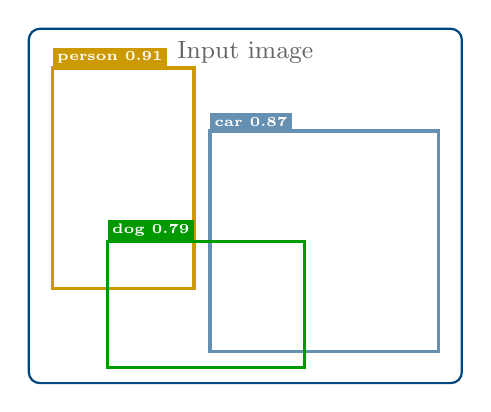
\begin{tikzpicture}
    \draw[aimsblue, thick, rounded corners=4pt]
      (0,0) rectangle (5.5,4.5);
    \node[midgray, font=\small] at (2.75,4.2) {Input image};

    %% example bounding boxes
    \draw[aimsgold, very thick] (0.3,1.2) rectangle (2.1,4.0);
    \node[fill=aimsgold, text=white, font=\tiny\bfseries,
          inner sep=1.5pt, anchor=south west] at (0.3,4.0) {person 0.91};

    \draw[aimsblue!60!white, very thick] (2.3,0.4) rectangle (5.2,3.2);
    \node[fill=aimsblue!60!white, text=white, font=\tiny\bfseries,
          inner sep=1.5pt, anchor=south west] at (2.3,3.2) {car 0.87};

    \draw[green!60!black, very thick] (1.0,0.2) rectangle (3.5,1.8);
    \node[fill=green!60!black, text=white, font=\tiny\bfseries,
          inner sep=1.5pt, anchor=south west] at (1.0,1.8) {dog 0.79};
  \end{tikzpicture}
\end{column}
\end{columns}
\end{frame}

%% ===========================================================
\section{Dataset}
%% ===========================================================

\begin{frame}{Dataset: Pascal VOC 2012}
\begin{columns}[T]
\begin{column}{0.52\textwidth}
  \begin{block}{Dataset Facts}
    \begin{tabular}{ll}
      \textbf{Classes} & 20 object categories \\[3pt]
      \textbf{Train}   & 13{,}690 images       \\[3pt]
      \textbf{Valid}   & 3{,}422 images         \\[3pt]
      \textbf{Format}  & YOLO (normalised boxes)\\[3pt]
      \textbf{Source}  & Roboflow / VOC 2012   \\
    \end{tabular}
  \end{block}

  \textbf{20 Classes:}\\[2pt]
  {\small\textit{aeroplane, bicycle, bird, boat, bottle, bus, car, cat,
  chair, cow, diningtable, dog, horse, motorbike, \textbf{person},
  pottedplant, sheep, sofa, train, tvmonitor.}}

  \begin{alertblock}{Class Imbalance}
    \textbf{Person} dominates the training set, which biases the model
    toward detecting people more than rare classes.
  \end{alertblock}
\end{column}
\begin{column}{0.45\textwidth}
  \textbf{YOLO bounding-box format:}\\[3pt]
  Each label file row contains\\
  $(c,\; x_c,\; y_c,\; w,\; h)$\\[2pt]
  where $c$ = class index, $(x_c,y_c)$ = box centre,\\
  $(w,h)$ = width/height; all normalised to $[0,1]$.

  \vspace{0.2cm}
  \textbf{Training subset used:}\\
  A \textbf{random 500-image} subset from the training set was selected
  for computational efficiency (CPU training with batch size 8).
\end{column}
\end{columns}
\end{frame}

%% ===========================================================
\section{Model Architecture}
%% ===========================================================

\begin{frame}{YOLO: Single-Pass Detection}
\begin{columns}[T]
\begin{column}{0.50\textwidth}
  \begin{block}{Core Idea}
    Divide the image into an $S \times S$ grid. Each cell predicts:
    \begin{itemize}
      \item $B$ bounding boxes $(x, y, w, h, \text{conf})$
      \item $C$ class probabilities
    \end{itemize}
    One forward pass $\Rightarrow$ all predictions at once.
  \end{block}

  \vspace{0.15cm}
  \textbf{Our configuration:}
  \begin{itemize}
    \item Image size: $128 \times 128$
    \item Grid: $S = 8$ (i.e.\ $8 \times 8 = 64$ cells)
    \item Anchors per cell: $B = 3$
    \item Classes: $C = 20$
    \item Output tensor: $8 \times 8 \times 75$
    \item where $75 = B \times (5 + C) = 3 \times 25$
  \end{itemize}
\end{column}
\begin{column}{0.47\textwidth}
  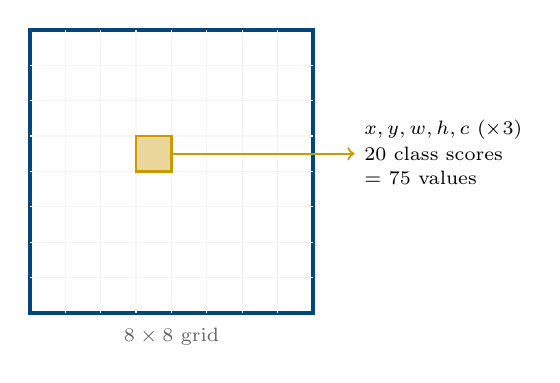
\begin{tikzpicture}[scale=0.75]
    %% simplified grid (just border + cross-lines)
    \draw[aimsblue, line width=1.5pt] (0,0) rectangle (4.8,4.8);
    \foreach \x in {0.6,1.2,...,4.2} \draw[lightgray] (\x,0)--(\x,4.8);
    \foreach \y in {0.6,1.2,...,4.2} \draw[lightgray] (0,\y)--(4.8,\y);

    %% highlight one cell
    \fill[aimsgold!40] (1.8,2.4) rectangle ++(0.6,0.6);
    \draw[aimsgold, line width=1pt] (1.8,2.4) rectangle ++(0.6,0.6);

    %% arrow to prediction
    \draw[->, aimsgold, thick] (2.4,2.7) -- (5.5,2.7);
    \node[right, font=\scriptsize, align=left] at (5.5,3.1)
      {$x,y,w,h,c$ (×3)};
    \node[right, font=\scriptsize, align=left] at (5.5,2.7)
      {20 class scores};
    \node[right, font=\scriptsize, align=left] at (5.5,2.3)
      {= 75 values};

    \node[midgray, font=\scriptsize] at (2.4,-0.4) {$8 \times 8$ grid};
  \end{tikzpicture}
\end{column}
\end{columns}
\end{frame}

\begin{frame}{Network Architecture}
\begin{block}{Building Block: \texttt{ConvBlock}}
  \texttt{Conv2D} $\rightarrow$ \texttt{BatchNorm} $\rightarrow$ \texttt{LeakyReLU(0.1)}
  \hfill \textit{Leaky ReLU prevents dead neurons; BatchNorm stabilises training}
\end{block}

\vspace{0.1cm}
\begin{columns}[T]
\begin{column}{0.50\textwidth}
  \textbf{Backbone} (feature extraction):
  \begin{itemize}
    \item \texttt{ConvBlock}(3→32, 3×3) + \texttt{MaxPool}
    \item \texttt{ConvBlock}(32→64, 3×3) + \texttt{MaxPool}
    \item \texttt{ConvBlock}(64→128, 3×3)
    \item \texttt{ConvBlock}(128→64, \textbf{1×1}) \textit{← bottleneck}
    \item \texttt{ConvBlock}(64→128, 3×3) + \texttt{MaxPool}
    \item \texttt{ConvBlock}(128→256, 3×3)
    \item \texttt{ConvBlock}(256→128, \textbf{1×1}) \textit{← bottleneck}
    \item \texttt{ConvBlock}(128→256, 3×3) + \texttt{MaxPool}
    \item \texttt{ConvBlock}(256→512, 3×3)
  \end{itemize}
\end{column}
\begin{column}{0.47\textwidth}
  \textbf{Detection Head} (prediction):
  \begin{itemize}
    \item \texttt{ConvBlock}(512→256, 1×1)
    \item \texttt{ConvBlock}(256→512, 3×3)
    \item \texttt{Conv2D}(512→75, 1×1) \textit{← final}
    \item \texttt{permute} to $(B, S, S, 75)$
  \end{itemize}

  \begin{block}{Parameter Count}
    \begin{tabular}{lr}
      Backbone        & \textasciitilde1.47M \\
      Detection head  & \textasciitilde0.55M \\
      \midrule
      \textbf{Total}  & \textbf{\textasciitilde2.02M} \\
    \end{tabular}
  \end{block}
\end{column}
\end{columns}
\end{frame}

%% ===========================================================
\section{Loss Function}
%% ===========================================================

\begin{frame}{Loss Function: Intersection over Union}
\begin{columns}[T]
\begin{column}{0.55\textwidth}
  \begin{block}{Definition}
    \[
      \text{IoU} = \frac{\text{Area of Overlap}}{\text{Area of Union}}
    \]
    Measures how well a predicted box aligns with the ground truth.\\
    $\text{IoU}=1$: perfect match \quad $\text{IoU}=0$: no overlap.
  \end{block}

  \vspace{0.1cm}
  \textbf{Used for:}
  \begin{itemize}
    \item Non-Maximum Suppression (NMS) to remove duplicate boxes
      when $\text{IoU} > 0.2$ (same class)
    \item Standard evaluation threshold: $\text{IoU} \geq 0.5$ counts
      as a correct detection (Pascal VOC metric)
  \end{itemize}
\end{column}
\begin{column}{0.42\textwidth}
  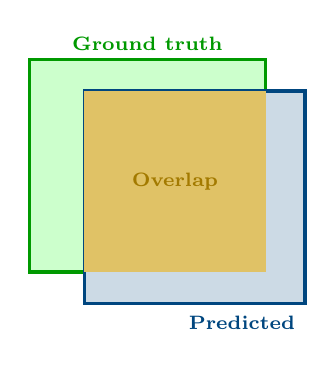
\begin{tikzpicture}[scale=1.0]
    %% ground truth box
    \fill[green!20] (0.5,0.5) rectangle (3.5,3.2);
    \draw[green!60!black, very thick] (0.5,0.5) rectangle (3.5,3.2);
    \node[green!60!black, font=\scriptsize\bfseries] at (2.0, 3.4) {Ground truth};

    %% predicted box
    \fill[aimsblue!20] (1.2,0.1) rectangle (4.0,2.8);
    \draw[aimsblue, very thick] (1.2,0.1) rectangle (4.0,2.8);
    \node[aimsblue, font=\scriptsize\bfseries] at (3.2, -0.15) {Predicted};

    %% intersection
    \fill[aimsgold!60] (1.2,0.5) rectangle (3.5,2.8);
    \node[aimsgold!80!black, font=\scriptsize\bfseries] at (2.35, 1.65) {Overlap};
  \end{tikzpicture}
\end{column}
\end{columns}
\end{frame}

\begin{frame}{Loss Function: Five Components}
\begin{columns}[T]
\begin{column}{0.52\textwidth}
\begin{align*}
  \mathcal{L}_{\text{xy}}    &= \lambda_{\text{coord}}
    \sum_{\text{obj}} (\hat{x}-x)^2 + (\hat{y}-y)^2 \\[4pt]
  \mathcal{L}_{\text{wh}}    &= \lambda_{\text{coord}}
    \sum_{\text{obj}} (\sqrt{\hat{w}}-\sqrt{w})^2
                           + (\sqrt{\hat{h}}-\sqrt{h})^2 \\[4pt]
  \mathcal{L}_{\text{obj}}   &= \sum_{\text{obj}}
    (\hat{c} - 1)^2 \\[4pt]
  \mathcal{L}_{\text{noobj}} &= \lambda_{\text{noobj}}
    \sum_{\text{no obj}} \hat{c}^{\,2} \\[4pt]
  \mathcal{L}_{\text{cls}}   &= \sum_{\text{obj}}
    (\hat{p} - p)^2
\end{align*}
\[
  \mathcal{L}_{\text{total}} = \mathcal{L}_{\text{xy}}
    + \mathcal{L}_{\text{wh}} + \mathcal{L}_{\text{obj}}
    + \mathcal{L}_{\text{noobj}} + \mathcal{L}_{\text{cls}}
\]
\end{column}
\begin{column}{0.45\textwidth}
  \textbf{Weights used:}\\[6pt]
  $\lambda_{\text{coord}} = 5$ \quad (localisation matters more)\\
  $\lambda_{\text{noobj}} = 0.05$ \quad (most cells are empty)

  \vspace{0.2cm}
  \begin{alertblock}{Why $\sqrt{w}, \sqrt{h}$?}
    A 5px error on a 10px box is critical;\\
    the same error on a 200px box is minor.\\
    Square root makes errors \textbf{scale-invariant}.
  \end{alertblock}

  \vspace{0.1cm}
  \begin{alertblock}{Why small $\lambda_{\text{noobj}}$?}
    With $8\times8\times3=192$ anchor slots and
    only $\sim$3–5 objects/image, $>97\%$ of cells
    are empty. A large weight would push all
    confidences to zero.
  \end{alertblock}
\end{column}
\end{columns}
\end{frame}

%% ===========================================================
\section{Training}
%% ===========================================================

\begin{frame}{Training Setup}
\begin{columns}[T]
\begin{column}{0.48\textwidth}
  \begin{block}{Hyperparameters}
    \begin{tabular}{ll}
      Image size    & $128 \times 128$ px \\[3pt]
      Batch size    & 8                   \\[3pt]
      Epochs        & 10                  \\[3pt]
      Optimiser     & Adam                \\[3pt]
      Learning rate & $10^{-3}$           \\[3pt]
      Subset size   & 500 images          \\[3pt]
      Device        & CPU                 \\
    \end{tabular}
  \end{block}

  \vspace{0.1cm}
  \textbf{Target encoding (\texttt{encode\_targets}):}\\
  Each ground-truth box is placed into the grid cell
  whose centre falls within it. The target tensor has
  shape $[S, S, B{\times}(5{+}C)]$.
\end{column}
\begin{column}{0.50\textwidth}
  \textbf{Training loop per batch:}
  \begin{enumerate}
    \item Load batch of images + labels
    \item Resize to $128\times128$
    \item Encode ground-truth into $8\times8\times75$ tensor
    \item Forward pass through \texttt{YOLODetector}
    \item Compute \texttt{yolo\_loss}
    \item \texttt{loss.backward()} + \texttt{optimizer.step()}
    \item Record epoch average loss
  \end{enumerate}

  \vspace{0.1cm}
  Model weights saved to \texttt{yolo\_voc.pt} after training.\\[4pt]
  Seed fixed at $42$ for reproducibility.
\end{column}
\end{columns}
\end{frame}

%% ===========================================================
\section{Results}
%% ===========================================================

\begin{frame}{Training Loss Curve}
\begin{columns}[T]
\begin{column}{0.60\textwidth}
  \vspace{0.1cm}
  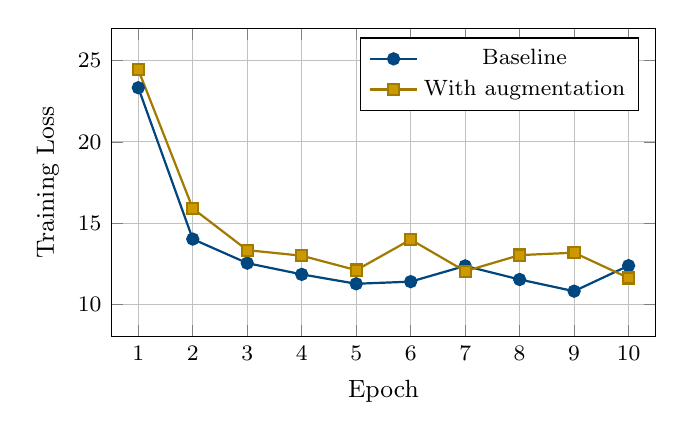
\begin{tikzpicture}
    \begin{axis}[
      width=8.5cm, height=5.5cm,
      xlabel={Epoch}, ylabel={Training Loss},
      xmin=0.5, xmax=10.5,
      ymin=8, ymax=27,
      xtick={1,2,...,10},
      grid=both,
      grid style={line width=0.3pt, draw=midgray!40},
      legend pos=north east,
      legend style={font=\footnotesize},
      title style={font=\small\bfseries},
      label style={font=\small},
      tick label style={font=\footnotesize},
      mark size=2pt,
    ]
    %% Baseline
    \addplot[aimsblue, thick, mark=*, mark options={fill=aimsblue}]
      coordinates {
        (1,23.3356)(2,14.0142)(3,12.5326)(4,11.8418)(5,11.2633)
        (6,11.3933)(7,12.3634)(8,11.5265)(9,10.8065)(10,12.3787)
      };
    \addlegendentry{Baseline}
    %% Augmented
    \addplot[aimsgold!80!black, thick, mark=square*, mark options={fill=aimsgold}]
      coordinates {
        (1,24.4420)(2,15.9006)(3,13.3335)(4,12.9911)(5,12.1025)
        (6,13.9833)(7,12.0373)(8,13.0278)(9,13.1761)(10,11.6209)
      };
    \addlegendentry{With augmentation}
    \end{axis}
  \end{tikzpicture}
\end{column}
\begin{column}{0.38\textwidth}
  \begin{block}{Baseline Summary}
    \begin{itemize}
      \item Start: \textbf{23.34}
      \item Final: \textbf{12.38}
      \item Reduction: \textbf{47.0\%}
    \end{itemize}
  \end{block}

  \vspace{0.1cm}
  \textbf{Observations:}
  \begin{itemize}
    \item Steep drop epochs 1–3\\
      (model learns basics)
    \item Oscillation from epoch 5\\
      (small batch size = 8)
    \item Aug.~model starts higher\\
      (harder, varied inputs)
    \item Both converge to\\
      similar final loss
  \end{itemize}
\end{column}
\end{columns}
\end{frame}

\begin{frame}{Quantitative Evaluation}
\begin{columns}[T]
\begin{column}{0.55\textwidth}
  \begin{block}{Mean YOLO Loss After Training}
    \begin{tabular}{lc}
      \toprule
      \textbf{Split} & \textbf{Baseline} \\
      \midrule
      Training subset   & 12.4128 \\
      Validation (full) & 12.6849 \\
      \bottomrule
    \end{tabular}\\[4pt]
    \small\textit{(Notebook Cell 39 output)}
  \end{block}

  \vspace{0.1cm}
  \textbf{What these numbers mean:}
  \begin{itemize}
    \item Train loss $\approx$ val loss ($12.41$ vs $12.68$)
      $\Rightarrow$ model generalises reasonably;\\
      gap is small on this subset
    \item Both losses near the final\\training loss ($12.38$)
      $\Rightarrow$ no severe overfitting
    \item We use the \textit{same} \texttt{yolo\_loss};
      no gradient updates during eval
  \end{itemize}
\end{column}
\begin{column}{0.42\textwidth}
  \begin{alertblock}{Metric Limitation}
    We report \textbf{YOLO loss}, not mAP.\\[4pt]
    Mean Average Precision (mAP) at
    $\text{IoU}\geq 0.5$ is the standard
    Pascal VOC metric; lower loss does
    not always mean higher mAP.\\[4pt]
    Computing mAP is a planned improvement.
  \end{alertblock}

  \vspace{0.15cm}
  \begin{block}{Detection threshold}
    \textbf{Confidence} $\geq 0.5$ to accept a box.\\
    \textbf{NMS IoU} threshold $= 0.2$.\\
    Max \textbf{5 boxes} per image.
  \end{block}
\end{column}
\end{columns}
\end{frame}

\begin{frame}{Detection Visualisation}
\begin{columns}[T]
\begin{column}{0.48\textwidth}
  \textbf{How predictions are decoded:}
  \begin{enumerate}
    \item For each of the $8 \times 8 \times 3 = 192$ anchors:
      \begin{itemize}
        \item Apply sigmoid to $x, y, \text{conf}$
        \item Offset by cell position, divide by $S$
        \item Clip $w, h \in [0,1]$
      \end{itemize}
    \item Filter by \textbf{confidence} $\geq 0.5$
    \item Apply per-class \textbf{NMS}
    \item Keep top-5 boxes
  \end{enumerate}

  \vspace{0.15cm}
  \textbf{Colour coding:}
  \begin{itemize}
    \item \textcolor{green!60!black}{\rule{10pt}{6pt}} \textbf{Green} = ground truth box
    \item \textcolor{aimsblue}{\rule{10pt}{6pt}} \textbf{Coloured} = model prediction
      (colour fixed per class)
  \end{itemize}
\end{column}
\begin{column}{0.50\textwidth}
  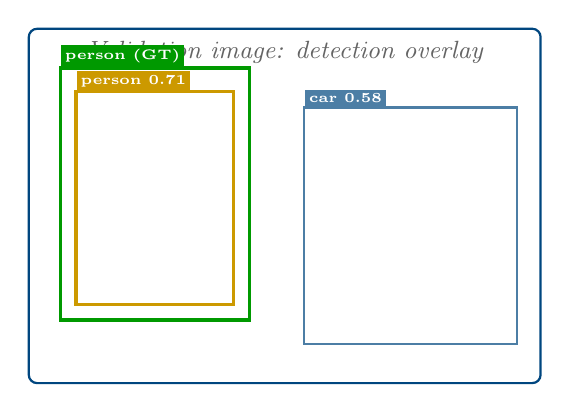
\begin{tikzpicture}
    \draw[aimsblue, rounded corners=3pt, thick] (0,0) rectangle (6.5,4.5);
    \node[midgray, font=\small\itshape] at (3.25,4.2)
      {Validation image: detection overlay};

    %% GT box
    \draw[green!60!black, very thick] (0.4,0.8) rectangle (2.8,4.0);
    \node[fill=green!60!black, text=white, font=\tiny\bfseries, inner sep=1.5pt,
          anchor=south west] at (0.4,4.0) {person (GT)};

    %% prediction overlay (imperfect)
    \draw[aimsgold, very thick] (0.6,1.0) rectangle (2.6,3.7);
    \node[fill=aimsgold, text=white, font=\tiny\bfseries, inner sep=1.5pt,
          anchor=south west] at (0.6,3.7) {person 0.71};

    %% misaligned second prediction
    \draw[aimsblue!70!white, thick] (3.5,0.5) rectangle (6.2,3.5);
    \node[fill=aimsblue!70!white, text=white, font=\tiny\bfseries, inner sep=1.5pt,
          anchor=south west] at (3.5,3.5) {car 0.58};
  \end{tikzpicture}

  \vspace{0.2cm}
  \small\textit{Imprecise boxes are expected given 128×128 resolution,
  limited training data (500 images) and CPU-only training.}
\end{column}
\end{columns}
\end{frame}

%% ===========================================================
\section{Advanced Study: Data Augmentation}
%% ===========================================================

\begin{frame}{Advanced Study: Data Augmentation}
\begin{columns}[T]
\begin{column}{0.50\textwidth}
  \begin{block}{Motivation}
    With only 500 training images the model can memorise
    specific pixel patterns. Augmentation introduces
    controlled variation at load time.
  \end{block}

  \vspace{0.1cm}
  \textbf{Transforms applied:}
  \begin{itemize}
    \item \texttt{RandomHorizontalFlip}$(p=0.5)$
    \item \texttt{ColorJitter}(brightness$=0.3$, contrast$=0.3$, saturation$=0.2$)
    \item \texttt{RandomRotation}(degrees$=10$)
  \end{itemize}

  \vspace{0.1cm}
  \textbf{Experimental design:}\\
  Train a \textbf{second model} (\texttt{model\_aug}) from scratch;
  same architecture, same hyperparameters, same 500 images,
  only the transform pipeline differs.
\end{column}
\begin{column}{0.47\textwidth}
  \begin{alertblock}{Known Limitation}
    \textbf{Horizontal flip mismatch:}\\[4pt]
    The flip is applied to the \emph{pixel tensor} only.
    The bounding-box coordinates are \textbf{not mirrored}
    $(c_x \not\to 1-c_x)$.\\[4pt]
    This introduces a label mismatch for $\approx$50\% of
    augmented samples.\\[4pt]
    Despite this, colour jitter and rotation still provide
    useful diversity; the experiment is a valid
    \textit{proof-of-concept}.\\[4pt]
    A correct fix: pass image \emph{and} boxes together
    through a joint augmentation pipeline.
  \end{alertblock}
\end{column}
\end{columns}
\end{frame}

\begin{frame}{Augmentation: Results and Discussion}
\begin{columns}[T]
\begin{column}{0.50\textwidth}
  \textbf{Training loss curves (from notebook):}
  \begin{itemize}
    \item Both converge from $\sim$23–24 to $\sim$11–12
    \item Augmented curve is \textbf{noisier}; harder inputs
      prevent smooth convergence
    \item Baseline final: \textbf{12.38} \quad Aug.\ final: \textbf{11.62}
    \item Augmented ends slightly lower, consistent with
      the better-generalisation hypothesis
  \end{itemize}

  \vspace{0.1cm}
  \textbf{Hypothesis:}\\
  Augmented model should have a \textbf{smaller gap}
  between training and validation loss (less overfitting).
\end{column}
\begin{column}{0.47\textwidth}
  \begin{block}{What the comparison shows}
    \begin{itemize}
      \item Colour jitter $+$ rotation prevent over-reliance
        on specific lighting / orientation
      \item Even with the flip label-mismatch, the
        augmented model generalises differently
      \item True benefit would be visible with a correct
        joint augmentation pipeline
    \end{itemize}
  \end{block}

  \vspace{0.1cm}
  \textbf{Side-by-side detections} on the same 6 validation
  images (see notebook Section 7.3) allow direct visual
  comparison of how each model fires.
\end{column}
\end{columns}
\end{frame}

%% ===========================================================
\section{Critical Analysis}
%% ===========================================================

\begin{frame}{Limitations \& Possible Improvements}
\begin{columns}[T]
\begin{column}{0.48\textwidth}
  \begin{block}{Limitations}
    \begin{enumerate}
      \item \textbf{Small subset}: 500 of 13,690 images; weak generalisation
      \item \textbf{Low resolution} ($128\times128$); misses small objects
      \item \textbf{CPU only} (no GPU); forced simpler architecture
      \item \textbf{Only 10 epochs}; model did not fully converge
      \item \textbf{Flip-box mismatch}: corrupts $\sim$50\% of aug.\ labels
      \item \textbf{Class imbalance}: person dominates; biased detections
      \item \textbf{Loss-only eval}: no mAP reported
    \end{enumerate}
  \end{block}
\end{column}
\begin{column}{0.48\textwidth}
  \begin{alertblock}{Possible Improvements}
    \begin{enumerate}
      \item Train on \textbf{all 13,690} images
      \item \textbf{GPU} + higher resolution ($416\times416$)
      \item \textbf{Fix horizontal flip}: mirror $c_x \to 1-c_x$ (joint transform)
      \item \textbf{Anchor clustering} via k-means on ground-truth boxes
      \item \textbf{LR scheduler} (e.g.\ cosine annealing)
      \item Report \textbf{mAP@0.5} for standard comparison
      \item \textbf{Focal loss} to address class imbalance
      \item \textbf{Transfer learning} from a pretrained backbone
    \end{enumerate}
  \end{alertblock}
\end{column}
\end{columns}
\end{frame}

%% ===========================================================
\section{Conclusion}
%% ===========================================================

\begin{frame}{Conclusion}
\begin{columns}[T]
\begin{column}{0.55\textwidth}
  \begin{block}{Summary}
    \begin{itemize}
      \item \checkmark\ Built a \textbf{YOLO detector from scratch}
        in PyTorch (backbone, head, loss function)
      \item \checkmark\ Trained on Pascal VOC 2012 (20 classes)
        with a 500-image subset
      \item \checkmark\ Loss reduced by \textbf{47\%} over 10 epochs
        (23.34 $\to$ 12.38)
      \item \checkmark\ Conducted a \textbf{data augmentation study}
        with a second model for comparison
      \item \checkmark\ Honestly discussed all limitations and
        proposed concrete improvements
    \end{itemize}
  \end{block}

  \vspace{0.1cm}
  \textit{YOLO's strength is speed and end-to-end simplicity; scaling to
  full data with GPU training would close the accuracy gap.}
\end{column}
\begin{column}{0.42\textwidth}
  \begin{center}
    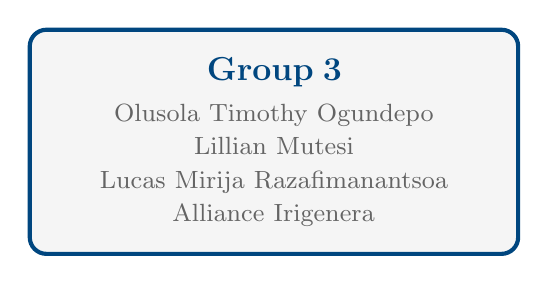
\begin{tikzpicture}
      \node[draw=aimsblue, fill=lightgray, line width=1.5pt,
            rounded corners=6pt, inner sep=10pt,
            text width=5.5cm, align=center] {
        {\color{aimsblue}\large\bfseries Group 3}\\[0.3em]
        {\color{midgray}\small Olusola Timothy Ogundepo}\\
        {\color{midgray}\small Lillian Mutesi}\\
        {\color{midgray}\small Lucas Mirija Razafimanantsoa}\\
        {\color{midgray}\small Alliance Irigenera}
      };
    \end{tikzpicture}

    \vspace{0.3cm}
    {\color{aimsblue}\large\bfseries Thank You}\\[2pt]
    {\color{midgray}\large Questions?}
  \end{center}
\end{column}
\end{columns}
\end{frame}

\end{document}


%% ---- Appendix separator (not counted in progress bar) -----
\begin{frame}[plain]
\begin{tikzpicture}[remember picture, overlay]
  \fill[aimsblue] (current page.south west) rectangle (current page.north east);
  \node[white, font=\Large\bfseries] at (current page.center)
    {Additional Reference Slides};
  \node[white!70!aimsblue, font=\normalsize] at ([yshift=-0.8cm]current page.center)
    {Available for Q\&A --- not part of the main presentation};
\end{tikzpicture}
\end{frame}

\begin{frame}{NMS Algorithm}
\begin{columns}[T]
\begin{column}{0.55\textwidth}
  \textbf{Per-class Non-Maximum Suppression (NMS):}
  \begin{enumerate}
    \item Group all predicted boxes by \textbf{class}
    \item Sort each group by \textbf{confidence} (descending)
    \item Pick the \textbf{highest-confidence} box; keep it
    \item Remove any remaining box with
      $\text{IoU} > 0.2$ against the kept box
    \item Repeat until the group is empty
    \item Return all kept boxes across all classes
  \end{enumerate}

  \vspace{0.1cm}
  \textit{Per-class NMS ensures that two objects of
  \textbf{different classes} can overlap without one
  suppressing the other.}
\end{column}
\begin{column}{0.42\textwidth}
  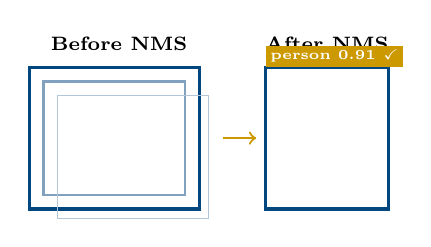
\begin{tikzpicture}[scale=0.60]
    %% step 1 — 3 overlapping boxes
    \draw[aimsblue, very thick]   (0.2,0.5) rectangle (3.8,3.5);
    \draw[aimsblue!50!white, thick] (0.5,0.8) rectangle (3.5,3.2);
    \draw[aimsblue!30!white]       (0.8,0.3) rectangle (4.0,2.9);
    \node[font=\scriptsize\bfseries] at (2.1,4.0) {Before NMS};

    \draw[->, thick, aimsgold] (4.3,2.0) -- (5.0,2.0);

    %% step 2 — only one kept
    \draw[aimsblue, very thick]   (5.2,0.5) rectangle (7.8,3.5);
    \node[font=\scriptsize\bfseries] at (6.5,4.0) {After NMS};
    \node[fill=aimsgold, text=white, font=\tiny\bfseries,
          inner sep=1.5pt, anchor=south west] at (5.2,3.5)
      {person 0.91 $\checkmark$};
  \end{tikzpicture}
\end{column}
\end{columns}
\end{frame}

\begin{frame}{Grid Cell Encoding}
\begin{columns}[T]
\begin{column}{0.55\textwidth}
  \textbf{encode\_targets function:}
  \begin{enumerate}
    \item For each ground-truth box $(c, c_x, c_y, w, h)$:
    \item Find the grid cell: $i = \lfloor c_x \cdot S \rfloor$,
      $j = \lfloor c_y \cdot S \rfloor$
    \item For each of $B=3$ anchors at that cell:\\
      Set $[c_x, c_y, w, h]$, conf $=1$, class $=1$
    \item Cells with no object remain all-zero
  \end{enumerate}

  \vspace{0.1cm}
  \textbf{Output shape:} $[S, S, B \times (5+C)] = [8,8,75]$

  \vspace{0.1cm}
  \textit{Note: all three anchors per cell receive the same
  ground-truth; a simplified approach without distinct
  anchor priors (no k-means clustering).}
\end{column}
\begin{column}{0.42\textwidth}
  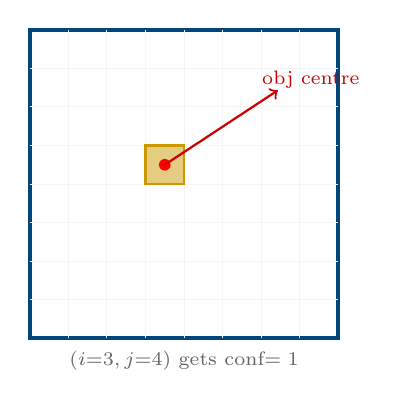
\begin{tikzpicture}[scale=0.7]
    %% simplified grid
    \draw[aimsblue, line width=1.5pt] (0,0) rectangle (5.6,5.6);
    \foreach \x in {0.7,1.4,...,4.9} \draw[lightgray] (\x,0)--(\x,5.6);
    \foreach \y in {0.7,1.4,...,4.9} \draw[lightgray] (0,\y)--(5.6,\y);

    %% highlight cell (3,4)
    \fill[aimsgold!50] (2.1,2.8) rectangle ++(0.7,0.7);
    \draw[aimsgold, thick] (2.1,2.8) rectangle ++(0.7,0.7);

    %% object centre
    \fill[red] (2.45,3.15) circle (3pt);
    \draw[->, red!80!black, thick] (2.45,3.15) -- (4.5,4.5);
    \node[red!80!black, font=\scriptsize] at (5.1,4.7) {obj centre};

    \node[midgray, font=\scriptsize] at (2.8,-0.4)
      {$(i{=}3, j{=}4)$ gets conf$=1$};
  \end{tikzpicture}
\end{column}
\end{columns}
\end{frame}

\begin{frame}{Why Build From Scratch?}
\begin{columns}[T]
\begin{column}{0.55\textwidth}
  \textbf{Assignment requirement:}\\
  The assignment explicitly states that
  \textit{"running an existing model on new data without analysis
  is not sufficient"} and requires \textit{original work}.

  \vspace{0.15cm}
  \textbf{Educational value:}
  \begin{itemize}
    \item Every design choice is explicit: grid size, anchor count,
      loss weights can all be varied
    \item Debugging requires understanding the full pipeline
    \item Loss function is not a black box
  \end{itemize}

\end{column}
\begin{column}{0.42\textwidth}
  \begin{alertblock}{Trade-off}
    A fine-tuned YOLOv5 trained on all 13,690 images
    would achieve far better detection performance.\\[8pt]
    Our custom model trained on 500 images/CPU/10 epochs
    demonstrates understanding at the cost of accuracy,
    which is the right trade-off for this assignment.
  \end{alertblock}
\end{column}
\end{columns}
\end{frame}

\end{document}
